\documentclass{article}
\usepackage[parfill]{parskip}
\usepackage[a4paper, total={6in, 9in}]{geometry}

\usepackage{titlesec}
\titlespacing*{\section}{0pt}{0.01\baselineskip}{0.01\baselineskip}

\usepackage{graphicx} %Paquete para incluir imagenes

\titleformat{\paragraph}
{\normalfont\normalsize\bfseries}{\theparagraph}{1em}{}
\titlespacing*{\paragraph}
{0pt}{3.25ex plus 1ex minus .2ex}{1.5ex plus .2ex}


\graphicspath{ {./images/} }
%\usepackage[margin=1cm]{geometry} % Centra el texto

\begin{document}

\begin{titlepage}
  \vspace*{1cm}

  \begin{center}
    {\Huge{Informe del Trabajo Practico 1}}
  \end{center}

  \vspace{0.4cm}

  \begin{center}
    {\LARGE{Facultad de Ingeniería de la Universidad de Buenos Aires}}\\
    \vspace{0.3cm}
  \end{center}

  \vspace{0.8cm}
  \begin{center}
    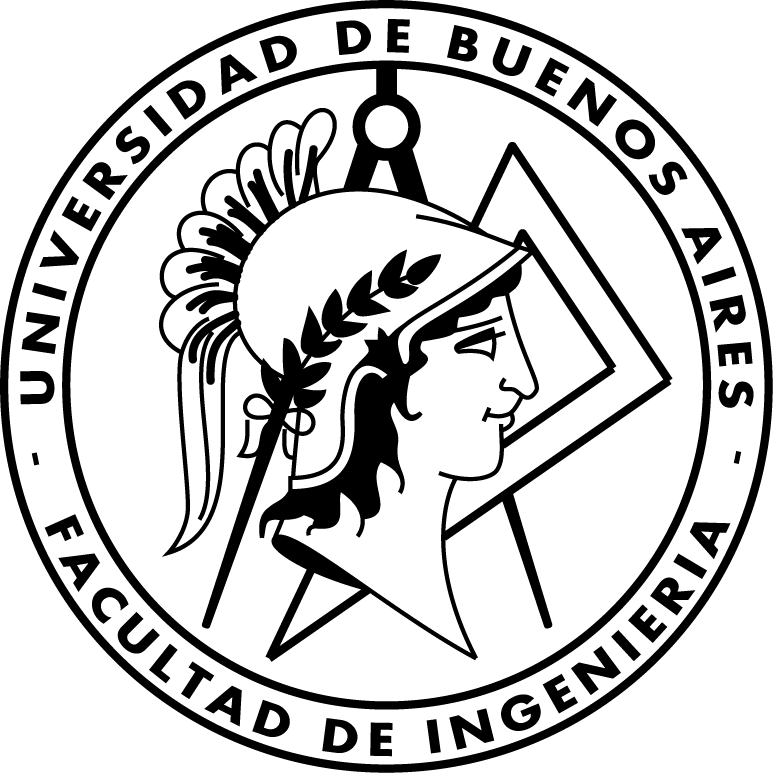
\includegraphics[scale=0.8]{Logo-fiuba}
  \end{center}

  \vspace{0.4cm}
  \begin{center}
    {\Large{Grupo 09}}\\
    \vspace{0.6cm}
    {\begin{minipage}[t]{.32\textwidth}
        \begin{center}
	Castro  Martinez, Jose Ignacio\\
          {\small{Padrón: 106957}}\\
          {\small{email: jacastrom@fi.uba.ar}}
        \end{center}
	\end{minipage}
	\begin{minipage}[t]{.32\textwidth}
        \begin{center}
	Douce, German Alejandro\\
          {\small{Padrón: 106001}}\\
          {\small{email: gdouce@fi.uba.ar}}\\
        \end{center}
      \end{minipage}
      \begin{minipage}[t]{.32\textwidth}
        \begin{center}
          Orsi, Tomas Fabrizio\\
          {\small{Padrón: 109735}}\\
          {\small{email: torsi@fi.uba.ar}}
        \end{center}
      \end{minipage}}
  \end{center}
\end{titlepage}

\section*{KNN} 

El modelo Knn es capaz de predecir con una precisión aceptable. Por un lado el modelo base tiene una precisión aproximada de 0.70, al someterlo a la búsqueda de hiperparametros y observar su comportamiento mientras se agregan más vecinos observamos que puede llegar a mejorar, de tal manera que toma una precisión aproximada de 0.74, lo cual representa una mejora considera con relación al modelo base. \\
El modelo no representa una mejora predictiva con relación al modelo anteriormente entrenado, el árbol de decisión. No se puede destacar tampoco la performance del modelo con relación a los modelos anteriores

\section*{SVM} 

Comenzamos este modelo probando los tres kernels (lineal, polinómico y radial) para ver cual era mejor Kernel. Resultó ser el Kernel lineal y nos dio un f1\_score de 0,75. Aun así decidimos probar por separado cada uno de los kernels. El lineal lo optimizamos pero no obtuvimos mejora en el score. 
El Kernel polinómico sin optimizar nos dio un score relativamente bajo (0,6). Al intentar optimizar sus hiperparametros, no pudimos terminar de correr el algoritmo debido al tiempo que tomaba. Los optimizamos a mano y obtuvimos una mejora (f1\_score 0,75).
Finalmente, el kernel radial sin optimizarlo nos dio un f1\_score muy bajo (0,60) y al optimizar hiperparametros apenas mejoró (0,67). Además para este caso no pudimos terminar de entrenar con CV para ver su capacidad de generalización.
Como conclusión de SVM, nos quedamos con el svm con kernel lineal debido a su performance y relativamente buen f1\_score (0,75)

\section*{Random Forest} 

Para el modelo random forest realizamos tres instancias. En la primera hicimos un modelo utilizando hiperparametros totalmente aleatorios. Para nuestra sorpresa, obtuvimos resultados bastante decentes (Un 80\% de precisión en el set de testeo).\\
Después de esto decidimos optimizar los hiperparametros del random forest con validación cruzada usando grid search optimizando la f1 score.  Estas optimizaciones implicaron una mejora del $\sim$ 3\% en el set de datos de testeos. Finalmente, decidimos hacer una optimización por validación cruzada con grid search buscando mejorar la mayor cantidad de métricas simultáneamente (precisamente: accuracy , f1 score, área bajo la curva roc, recall y precisión). A pesar de toda esta optimización, no hubo ninguna mejora considerable a la hora de predecir el set de testeo (solo hubo una mejora del $\sim$ 0.01). 

\section*{XGBoost} 

El modelo XGBoost representa el primer modelo que en su forma base genera la mejor predicción de todos los modelos entrenados en el análisis. Se realiza una búsqueda de los mejores hiperparametros, la cual, no genera una mejora consistente en las capacidades predictivas del modelo. Por lo tanto, se pueden llegar a las conclusiones que los modelos de ensambles usando árboles y los modelos de árboles son los más precisiones  la hora de realizar predicciones

\section*{Voting} 
Tanto para el ensamble voting como stacking, decidimos usar los mejores modelos que obtuvimos en las etapas anteriores. Esto lo hicimos para poder sacar el mayor jugo de los modelos que habíamos obtenido antes. \\
Sin embargo, para nuestra sorpresa, obtuvimos resultados peores que con los modelos por separado. Para tratar mejorar este resultado, eliminamos el modelo svm (el cual nos había dado malos resultados) y cambiamos el modelo de votación a una votación ponderada. Esto nos dio resultados mejores, pero no superior al XGBoost


\section*{Stacking} 
El modelo stacking fue entrenado con los distintos modelos producidos a lo largo del análisis tuvo una precisión menor a lo esperado, los modelos bases usados en su construcción tienen una precisión superior a la predicción global hecha por el modelo, por lo cual, consideramos que tiene buenas métricas pero no representa una mejora considerable a los resultados anteriormente mencionados.

\section*{General} 
En base a los resultados observados, se puede inferir que los modelos que emplean árboles de decisión presentan una adaptabilidad notable al generar predicciones sobre los datos. Sin embargo, es importante destacar que los demás modelos no muestran un rendimiento considerablemente inferior en comparación. Un problema que pudieron haber tenido nuestros modelos de ensamble híbrido, es que están usando modelos muy optimizados para sí mismos; esto puede haber introducido un sesgo alto. 

\end{document}
